\documentclass[UTF8, 11pt, oneside]{ctexart}

\usepackage{float}

\usepackage{geometry}
\geometry{a4paper,left=2cm,right=2cm,top=2cm,bottom=1cm}

\usepackage{graphicx}

\usepackage{hyperref}
\hypersetup{colorlinks=true, linkcolor=red}

\linespread{1.6}


\def\articletitle{混血劣势的宝宝,你敢和外国人生吗?}

\usepackage{fancyhdr}
\usepackage{ifthen}
\pagestyle{fancy}
\fancyhf{}
\setlength{\headheight}{14pt}
\fancyhead[R]{\ifthenelse{\value{page}>1}{\thepage}{}}
\fancyhead[C]{\ifthenelse{\value{page}>1}{\articletitle}{}}
\renewcommand\headrulewidth{0pt}

\usepackage{tcolorbox}
\tcbuselibrary{skins}


\newcommand{\zd}[1]{\textbf{\textcolor[RGB]{123,12,0}{#1}}} % 重点

\newcommand{\yh}[1]{% 引用
    \begin{tcolorbox}[enhanced,
        frame hidden, interior hidden,
        before skip = 5mm, left skip=10mm,
        borderline west={5pt}{0pt}{gray!50}]
        #1
    \end{tcolorbox}
}

\newcommand{\biaoti}[1]{% 标题
    \section*{#1}
}

\begin{document}

\begin{center}
    \LARGE{\articletitle\footnotemark}
\end{center}
\footnotetext{
    原文出自公众号“远方青木”的文章 《\href{https://mp.weixin.qq.com/s/5KbdFk6M7UrMW8NMgyDIBg}{\articletitle}》
}

100多年来,中国太弱了,各种殖民思维长期统治着中国大地。

我长期致力于驱除笼罩在中国的隐形殖民思维,但这个工作实在太艰难,工作量实在太大了,于是我只能一点点来。

\zd{今天,我要破除的谣言就是混血优势,这个谣言长期以来欺骗了无数的中国人,殖民了不少中国人的思想。}

之所以我今天要谈这个,是因为看到了今天无数人热捧一个未婚生育,买下英国白人精子怀孕的女模特。

\begin{figure}[H]
    \centering
    
\includegraphics[width=10cm]{2023-03-30-001}
\end{figure}

女人想未婚生育,那是自己的自由,只要自己赚够钱,想过什么样的日子都可以,但我看到舆论场上无数不知道哪来的小号话里话外都是白人男子精子更优秀,中国男人都是劣等精子之类的言论时就非常生气。

\zd{传播谣言是违法的,你们知道吗?}

\zd{恶意攻击中国形象,攻击中国自信的根基也是违法的,你们知道吗?}

碰巧,我又看到了下面这个新闻截图,我就更生气了。

\begin{figure}[H]
    \centering
    
\includegraphics[width=10cm]{2023-03-30-002}
\end{figure}

说这种话的,还是中国人?是不是跪在地上太久,以至于起不来了?

\zd{思想被洗脑到这个地步的人,已经不配当中国人了,不管是男是女。}

\zd{混血优势的谣言一日不破除,中国人的膝盖一日跪在地上起不来。}

天天张口闭口混血优势,混血宝宝漂亮聪明,那你知道什么是混血劣势吗?

你听说过\zd{混血劣势}这个词吗?知道二战前的科学家关于混血劣势出了多少篇科学文献吗?你什么都不知道,因为这个词被欧美霸权给强行抹除了,不允许主流舆论提及。

\zd{关于混血劣势,全世界的主流舆论全部失声,列为禁忌,默契的封杀了70多年。}

本来这个词我们中国媒体也不应该提,因为政治不正确,不利于开放和交流,但鉴于欧美利用混血优势的理论殖民中国人的思想,我不得不把这个科学词汇拿出来科普。

\zd{虽然有那么一点点政治不正确,但混血优势的谣言太难破除,没什么好办法,只能拿这个来以毒攻毒。}

首先,有没有混血优势,或者说混血能否产生优秀的宝宝。

答案是可以,混血优势并不算完全的谣言,混血确实会大幅提升诞生顶级优秀宝宝的概率,这个原理和水稻领域的杂交育种是一致的。

\zd{但你因此就简单粗暴的得出混血是好事,那就大错特错了。}

你有没有思考过,为什么混血会大幅提升诞生顶级优秀宝宝的概率?

你身上有100条基因,找的对象也有100条基因,混合后诞生的宝宝也是100条基因。

一条基因没多,为什么后代会更优秀?

因为男女婚配诞生后代,本质上是把两个人的基因组给拆散后进行重组,你出50条基因,对象出50条基因,重组成一个100条基因的宝宝。

无论你是纯血宝宝还是混血宝宝,都是这个生殖流程。

但你和你对象的种族差距越大,你们基因组的差距就会越大,你们分别拥有不同优势基因的概率就越大。

在重组的过程中,极其幸运的孩子,有可能会同时继承你们两人的优势基因,从而诞生一个稀有的拥有双优势特性的宝宝,这是纯血宝宝不可能做到的,因为纯血宝宝最多单优势。

所以,这个叫混血优势,杂交育种领域就通过这种手段不断的杂交,把不同的优势基因聚合在一个种子身上,从而诞生一个无敌种子。

听起来好像是好事啊,而且是极好的事情。

但你有没有想过,虽然每个人身上都有优势基因,但同时也有劣势基因。

杂交有概率聚合优势基因,同时也会有概率聚合劣势基因。

混血后,有概率诞生一个奇差无比的宝宝,远远低于正常生育的平均值。

\zd{这个,就叫混血劣势。}

而且还不止如此,优势基因需要完全聚合才能体现出混血优势,激发概率极小,但混血劣势却非常容易触发。

因为当人类宝宝达到优秀线以上的时候,你多聚合一条优势基因这看不出来什么。

但那些劣势基因,只要聚合一条就是天大的问题。

脸上长胎记的宝宝你能接受吗?

天生白化病的宝宝你能接受吗?

出生就残一条腿的宝宝你能接受吗?

先天心脏病的宝宝你能接受吗?

\zd{不需要完全聚合如此之多的劣势基因,只要激活一条,你这宝宝的人生就会灰暗无比。}

\zd{而混血,会导致进入重组基因库的劣势基因直接翻倍,激活某个劣势基因的概率也直接翻倍。}

混血宝宝激活单个劣势基因的概率,比聚合多条优势基因的概率,那要直接大几百倍。

而对于人类社会来说,你生出来就必须要养,而且要费尽心血给激活的劣势基因的宝宝继续找对象,不然你于心不忍。

\zd{从整个人类社会的角度来说,混血是绝对劣势,诞生出的个别优势宝宝,完全不能抵消诞生的大量劣势宝宝所引发的社会的负担。}

那为什么育种工作要大量的采用杂交手段,诞生出的大量劣势种子应该怎么办?

简单,毁灭掉就可以了,那只是个种子而已。

毁掉一万个乃至于十万个失败的种子,只要能获得一个我需要的优势种子,那就算我成功了。

\zd{失败的劣势水稻种子你可以随便毁掉,失败的劣势人类宝宝,你能毁掉吗?}

\zd{所以水稻育种能用的手段,人类社会不能用。}

除了混血劣势理论外,遗传届还有个更黑暗的理论,那就是纯血育种理论。

和杂交育种完全反过来,纯血育种理论是通过近亲繁殖,反复纯化和提取某种优势基因,从而获得纯化良种。

杂交育种的混血优势,不一定是优势,这么育种最大的作用在于重组基因,引入一个你需要的基因。

比如说中国人的孩子皮肤永远黄的,你怎么生育都不会变黑。

如果你想获得黑皮肤的基因,你就必须引入黑人的基因。

水稻的杂交育种也是一样,杂交的目的其实是引入一些抗倒伏,抗病基因等,并不是说我舍得淘汰十万个失败种子就一定可以获得一个优势种子。

杂交前,要精心选择父本和母本,确定好你的杂交目的,你需要同时聚合父本和母本身上的那些优势基因,然后才会开始进行杂交育种工作。

这个才叫科研,科研并不是随机撞大运。

一旦培育出了自己需要的种子,同时聚合了自己所需的所有基因,那下一步应该怎么办?

纯化,反复的纯化,通过近亲繁殖反复纯化稳定这些基因组,最终获得一个可以稳定同时遗传这些基因的纯血种子。

当然,在实际育种工作中,为了保护知识产权,保证种子公司的利益,科研工作者一般都是通过近亲繁殖反复纯化父本和母本,获得纯化父本母本后,稳定生产杂交一代。

杂交一代性状非常优秀,优势基因完全聚合,但杂交二代一定基因混乱,长的乱七八糟,确保你每年都要买他家的种子,这就是育种公司保护自己的手段。

换句话说,在育种工作中,近亲繁殖是一个非常重要且常见的手段,这个手段可以轻易聚合优势基因,其理论基础是和混血杂交完全相反的。

如何解释近亲繁殖带来的基因优势?

因为基因和基因之间是不平等的,有些基因被人类认定为优质基因,有些基因被人类认定为劣质基因。

当某个体身上忽然突变出一个特别好的优势基因时,他的后代是未必可以继承这种基因的。

\zd{如果你想以后代代都有这种优势基因,最佳办法绝对不是混血,而是让此个体近亲繁殖,不断的纯化提取这个优势基因,最终获得一个可以稳定遗传此优势基因的后代。}

再举个例子,在宠物育种领域,假设你认定贵宾犬的外表是优势基因,吉娃娃的外表是劣势基因。

那么对于贵宾犬而言,最佳的育种手段绝不是和吉娃娃混血,而是和另一个贵宾犬繁殖。

再进一步,当你拥有一个特别漂亮的贵宾犬时,如果你想繁殖出更多的和它一样漂亮的贵宾犬应该怎么办?

漂亮贵宾犬的后代不一定漂亮,有漂亮有不漂亮的,尤其是和不同犬只配种之后,生下来的小狗更是千差万别。

在宠物育种届,碰到这样的漂亮种犬,为了自身利益最大化,采取的手段非常黑暗。

他们让这只漂亮贵宾犬疯狂的近亲繁殖,甚至是母子繁殖,不断纯化提取那个漂亮基因,最终获得一个可以稳定生育漂亮贵宾犬的小家族。

近亲繁殖时,相同的优势基因会轻易表现出来,从而打造出优秀的纯血个体,达到选育的目的。

但同样,近亲繁殖也会导致相同的劣势基因轻易表达出来,从而打造出残疾、患病的劣势个体。

近亲繁殖容易生下残疾宝宝,这是基础知识,那为何还有宠物贩子让纯血优秀个体不断的近亲繁殖?

很简单,生下的优秀狗宝宝,可以卖出大价钱。

万一生出了残疾、患病的狗宝宝,直接“处理”掉便是。

很多爱狗人士购买的漂亮纯血狗宝宝,就是通过这种手段批量制造出来的。

\zd{可惜,狗贩子育种场里的黑暗,他们看不到。}

\zd{劣势的狗宝宝可以随便处理掉,劣势的人宝宝你能处理吗?}

\zd{所以,宠物育种可以用近亲繁殖的手段,人类社会不行。}

但是在纯化优势基因领域,近亲繁殖确实是非常有效的手段,只不过因此带来的残缺婴儿的巨大代价,人类社会实在是无法承受。

人类社会经过研究,反复对比利害关系,最终禁止了三代以内的近亲繁殖。

以前还可以表兄妹结婚,但现代社会绝对不允许了。

三代以内的婚配,表兄妹乃至于亲兄妹结婚,后代纯化优势基因的概率远远高于正常人,但同时纯化劣势基因的概率也远远大于正常人。

人类社会认定,三代以内的婚配弊大于利,除非你抛弃人权,直接淘汰缺陷儿,只留健康宝宝。

\zd{如果必须要抚养缺陷儿,那三代以内就不能婚配,否则纯化优势基因的作用是没有意义的。}

通过混血手段来提取优势基因的利弊分析,也是这样。

\zd{混血确实有概率聚合优势基因,诞生极优秀宝宝,但同时也会导致劣势基因表达的概率大幅增加。}

\zd{除非你敢于淘汰缺陷儿,否则从人类社会整体角度而言,是没有什么好处的,甚至是弊大于利。}

尤其是在你假定本族基因最优秀,其他人种的基因都略弱于本族基因时,混血劣势会被无限放大,从而导致严重的弊大于利。

二战前,关于混血优势和劣势的争论持续了很久,最终各国科学家得出的结论是混血没有优势,反而是劣势。

这个结论直接导致了二战前期各国对外族人口的排外行为,而世界上最大的混血国美国被认定为劣势基因的大杂烩,全球最弱的民族。

希特勒大力推行纯种雅利安人策略,和德国科学家认定混血劣势,认定混血弊大于利有直接关系。

同时,希特勒在二战前期非常看不起美国人的战斗力,认定美国是一个稀烂而软弱不堪的种族,也和混血劣势论有直接关系。

最后,二战是美国赢了,然后美国支配了这个世界。

\zd{美国是一个移民国家,世界上最大的混血国,你说美国能容忍混血劣势论这种研究成果存在?}

所以,二战后,美国通过舆论把混血劣势论和德国的种族大屠杀绑定,认定德国发动大屠杀就是因为混血劣势论。

从此,谁敢提混血劣势论,谁就会被打成纳粹,这个理论在全球舆论界被封杀了整整70多年。

\zd{美国只允许提混血优势论,以此来证明自己的国家是世界上最优秀的国家,并在全世界反复强调和固化这一理论。}

本来吧,你鼓吹混血优势论也行,中国不介意这个。

\zd{但你不能拿这套东西来洗脑中国人,殖民我们的思想。}

在欧美舆论的操纵和潜移默化的暗示下,混血优势被默认成和白人混血才有优势。

和黄种人混血是没有优势的,和黑种人混血是没有优势的,只有和白种人混血才有优势。

你可以回顾下你的潜意识,在被混血优势论洗脑后,你会认为和黑种人混血产生的宝宝很优秀吗?

不会的,你会下意识的反感,同时只会认为自己和白种人混血宝宝很优秀。

\zd{不是混血优势吗?怎么和黑人混血就没优势?怎么和黑人混血就会产生一个智商低,各种毛病的孩子呢?}

\zd{你怎么不好好想一想,哪怕混血优势论是正确的,你也不应该产生这种思维啊。}

\zd{还有更离谱的,和白人混血优势,又被默认为中国女人和白种男人的混血。}

\zd{简单的说,欧美利用舆论洗脑,成功的让中国人相信中国和欧美混血可以产生优势宝宝,但欧美人不相信和中国人混血可以产生优势宝宝。}

假定和白人混血会产生优势宝宝的理论是正确的,那为了获取一个优势宝宝,白种人应该疯狂的和中国人通婚啊,白种男拼命的追求中国女人,白种女拼命的追求中国男人。

但事实上,白种人对和中国人通婚兴致缺缺,对混血宝宝毫无兴趣,但中国人却对白人混血兴趣高昂,认定混血优势。

\zd{亲,人家自己都不相信和你混血能产生优势,你凭什么这么信?}

欧美舆论是通过何等鬼斧神工的手段,能让同一套理论在不同的国家产生不同的效果。

\zd{鼓吹混血优势论很简单,但让中国人信而欧美人不信,这就很难了,你又不能明说这个是假的。}

\zd{要信一起信,要不信就一起不信。}

\zd{怎么才能做到只让一方相信?而且信到死,铁杆信徒那种,同时让另一方不信?}

是不是不可思议?

但人家欧美舆论做到了。

手段其实不难,因为欧美舆论从来就不提混血优势。

你可以去查阅所有新闻,欧美媒体从来就不提混血优势论,提混血优势的全部是中国媒体。

在自己不提混血优势论的基础上,如何做到让中国媒体主动提这个?

也很简单。

利用幸存者效应。

\zd{幸存者效应是欧美舆论特别喜欢用的一个手段,覆盖几乎所有领域,是欧美舆论洗脑全世界的最重要武器。}

\zd{不管是宣传欧美体制,欧美经济,欧美文化,他们都会反复利用幸存者效应。}

以混血宝宝为例,混血宝宝产生缺陷的概率会大大提升,但确实有聚合优势基因的作用。

因此,在成千上万的混血宝宝里,一定会出现一个很漂亮的混血宝宝,这是有科学根据的。

当这样的宝宝出现时,其他几百几千个劣势宝宝直接全部忽略,假装他们不存在于这个世界,把镜头对准那个优势宝宝,给与TA大量的曝光和关注度。

然后,反复强调这个宝宝是混血的,诱导人们把这个宝宝漂亮的原因认定为中美混血导致。

当然,玩这一套的前提条件,是这个宝宝位于中国,或者是中国女性和美国男性的混血。

如果是中国男性和白人女性的混血漂亮宝宝,则忽略不提,假装这个宝宝不存在。

如果这个漂亮混血宝宝位于美国境内,那宣传就更简单了。

\zd{记住,在中国如果出现漂亮混血宝宝,那欧美媒体会强调这是一个混血宝宝。}

\zd{在美国如果出现漂亮混血宝宝,那欧美媒体会强调这是一个美国宝宝。}

\zd{如果出现丑陋的混血宝宝,则任何时候都绝口不提。}

看清楚这里面的门道了吗?

我根本不用宣传什么混血优势论,我只需要这么春秋笔法的反复宣传个十几年,我想要的一切目的都会实现。

\zd{这个,叫文化入侵,文化殖民。}


因此,欧美媒体才可以鬼斧神工的把混血优势论换成黄白混血优势论,且只让黄种人,甚至只是黄种女人相信。

\zd{这本质上,是在鼓吹白种人基因优势论,而不是混血优势论,是欧美文化自信,种族自信,制度自信建设的一部分。}

\zd{你和我混血会产生优势宝宝,而我和你混血不会产生优势宝宝。}

\zd{所以你是劣质人类,我是优质人类,这个推论有问题吗?}

\zd{因为我是优质人类,所以我的国家是优质的,我的文化是优质的,我的种族是优质的,而你的一切都是劣质的,这有问题吗?}

\zd{我说这属于殖民入侵,破除这种谣言是我作为中国人应肩负的义务,这有问题吗?}

来点文化自信的内容给大家科普一下。

现代科学家对世界三大人种的脑容量进行了研究,发现三大人种的脑容量有明显区别。

成年后,东亚人的脑容量,平均值比白种人多出1立方英寸,而白种人又比黑种人多5立方英寸。

这不是啥理论,是纯粹的事实,东亚人的脑容量平均值就是要大很多。

\begin{figure}[H]
    \centering
    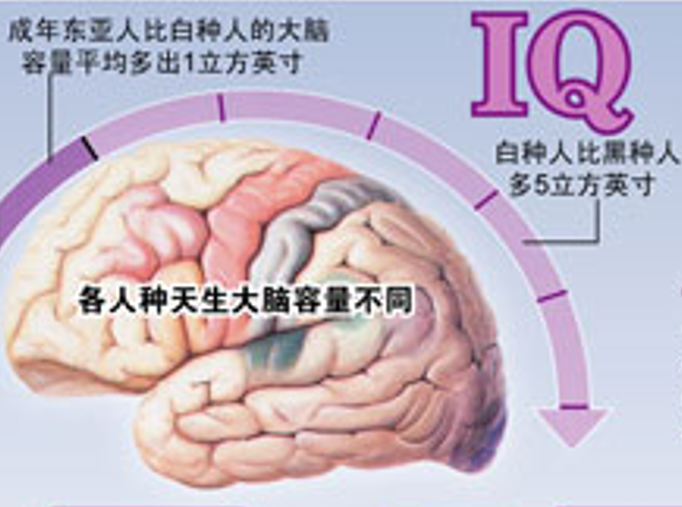
\includegraphics[width=10cm]{2023-03-30-003}
\end{figure}

而对各人种的智商测试发现,东亚地区的IQ测试平均值为106,白种人约为100,美国黑种人为85,撒哈拉地区的非洲黑人为70。

\begin{figure}[H]
    \centering
    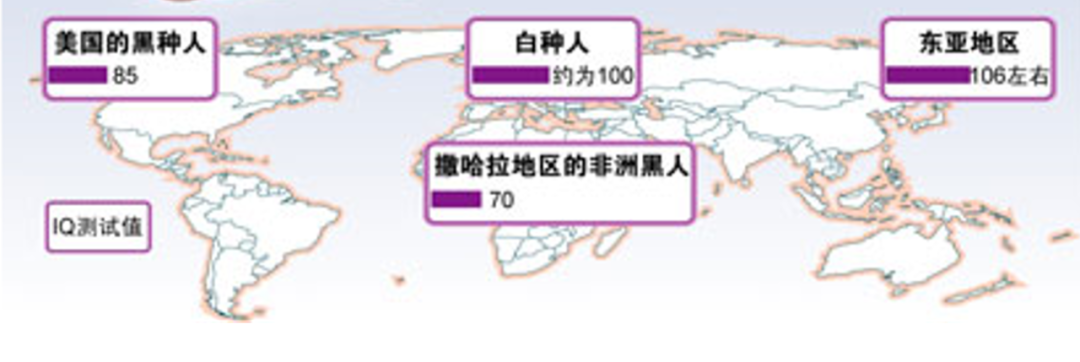
\includegraphics[width=10cm]{2023-03-30-004}
\end{figure}

当然,黑人也不是一无是处,研究发现黑人儿童学坐、爬、走和穿衣服的时间比白人和东亚人都要快,运动方面的天赋明显比东亚人强一截。

\zd{但如果只论脑容量和智商,黑人明显不行,连白人都比东亚人差一丝。}

而对于混血儿的智商,科学家也有研究。

世界上最大的混血国并不是美国,而是中美洲地区,这里曾残存大量的印第安人,大量的印第安女人和白种男人混血。

因此,这里成为了研究混血的最佳样本地区。

假定混血可以提高种族素质,批量诞生优势宝宝,那中美洲地区应该是世界上最富强的国家,碾压欧洲,碾压美国,更是远远碾压中国。

但实际上,这里穷困不堪,混乱不已。

墨西哥离美国那么近,提前发展了那么多年,如今哪怕只论人均GDP都不如中国,而且毒品和凶杀横行,国家看不到未来。

至于中美洲的其他国家,还不如墨西哥,更惨。

由于黑人IQ明显低黄白人种一截,而印第安人属于黄种人,所以单纯从研究智商方面,黑白人种更有利于看出基因的重分布情况。

南非就是一个很好的样本,这个国家黑白混血儿大量存在。

研究结果表明,黑白混血儿的平均IQ,基本恰好等于白种人和非洲黑人IQ的平均值。

\begin{figure}[H]
    \centering
    
\includegraphics[width=10cm]{2023-03-30-005}
\end{figure}

从以上数据我们可以得出结论,混血带来的是基因重分布,谈不上优势还是劣势。

只论智商,那基本就是直接来个父母平均。

\zd{但如果从缺陷基因表达导致缺陷儿的概率层面来说,混血是劣势的,诞生缺陷儿的概率远远大于你期望的优势基因聚合体出现的概率。}

\zd{虽然总体是平衡的,但如果你把每一个缺陷基因单独表达的孩子都视为“负担”的话,那混血对于社会整体来说是弊大于利的。}

如果你不介意大量缺陷宝宝的诞生,非要去摸彩票,赌优势基因聚合体的话,那你为什么不直接近亲繁殖呢?纯化自身优势基因的概率要大的多。

\zd{难不成,你自认为自己的基因是劣质的,没有丝毫纯化自身基因的兴趣,只想着通过混血改造下自己的劣质基因?}

\zd{如此自轻自贱之人,还指望别人会尊重你吗?}

马和驴混血的后代,是骡子,连生育能力都没有。

但你见过哪个欧美女性,天天狂热的跑到中国要和中国男性混血?

因为人家早就尝试过了,也做过大量混血尝试,事实证明混血儿压根没有任何优势,甚至弊大于利,所以欧美人对和中国人混血没有丝毫兴趣。

如果混血儿的智商一定比父母平均值增长1,那么1000代下来人类智商早就被提升到1000了,但这样的超级人类连影都没见到。

混血对于提升种族智商丝毫用处都没,但这并不介意他们通过潜移默化的手段来忽悠中国人,让一部分中国人认定混血优势论,在心态上被殖民,默认自己低欧美一等。

也许有人认为欧美人鼓吹这个,是为了轻易骗取大量中国女人。

这么想你就狭隘了,欧美人这么麻烦的宣传这种理论,可不是为了区区几个女人。

\zd{让中国人承认自己基因劣质,人种劣质,文化劣质,制度劣质,国家劣质,这才是鼓吹混血优势论的主要目的。}

\zd{一切宣传的终极目的,都是这个。}

在育种领域,近亲繁殖和混血杂交都可能会诞生优质后代,但代价就是会出现无数的缺陷后代和劣质宝宝。

这个代价在育种领域可以承受,但人类社会无法承受。

无法放弃缺陷宝宝,那这套婚配办法就会产生巨大的问题。

因此,科学家把这个称之为混血劣势。

自从美国在二战中胜出后,混血劣势理论已经被封杀了70年。

但混血的代价确实很大,丑陋缺陷儿的概率远大于优质宝宝的概率,对于社会整体而言是弊大于利的。

\zd{混血劣势的宝宝,你敢和外国人生吗? }

\zd{你哪来的自信自己一定能中彩票呢?默认自己一定是幸存者。}

\zd{就好像国内那些二鬼子,你哪来的自信美国一定给你发绿卡呢?}

\zd{美国每年给一点点幸存者发绿卡,你凭什么以为你就可以这么幸运?}

如果美国愿意要你,愿意给你绿卡,愿意给你发美国工资,那你赶紧走,中国绝不阻拦你,别在中国这天天鼓吹白人基因优质论。

问题是,你美国爹他不愿意发给你啊,这东西本来就是美国丢出来的骨头,每年挑少数一点幸运儿给,用幸存者效应来树立美国文化自信,体制自信用的。

东亚人脑容量世界第一,智商平均值世界第一,这是科学事实,记住了吗?

\zd{记不住,就麻烦你赶紧去美国,换美国国籍,好好当一个美国人。}

\zd{就怕美国觉得你很劣质,从基因到人品都很劣质,怕被你污染,不允许你当美国人,那就尴尬了。}

\end{document}

